\documentclass[sutton_barto_notes.tex]{subfiles}

\begin{document}


\newpage
\section{Dynamic Programming}

In RL, DP refers to a collection of algorithms that can be used to compute optimal policies $\pi_*$ given a perfect model of the environment as a Markov decision process (MDP).
DP itself cannot be useful in RL due to its computational cost and requirement of a perfect model, but DP provides an essential foundation for the understanding of other algorithms.
Other algorithms can be treated as attempts to achieve much the same effect as DP, only with less computation and without assuming a perfect model of the environment.

Starting with this chapter, we assume the environment is a finite MDP (i.e. $S$, $A$, $R$ are finite and dynamics are given by a set of probabilities $p(s',r|s,a)$).
A common way of obtaining approximate solutions for tasks with continuous states and actions is to quantize the state and action spaces and then apply finite-state DP methods.
In this chapter we show how DP can be used to compute the value functions defined in Chapter 3. As shown in Chapter 3, we can obtain $\pi_*$ once we have found $v_*$ or $q_*$, which satisfy the Bellman optimality equations:

\begin{align*}
v_*(s) & = \max_a \E [R_{t+1} + \gamma v_*(S_{t+1}) | S_t = s, A_t = a] \\
& = \max_a \sum_{s',r} p(s',r|s,a)[r + \gamma v_*(s')]
\end{align*}

\begin{align*}
q_*(s,a) & = \E [R_{t+1} + \gamma \max_{a'} q_*(S_{t+1},a') | S_t = s, A_t = a] \\
& = \sum_{s',r} p(s',r|s,a)[r+\gamma \max_{a'} q_*(s',a')]
\end{align*}

\subsection{Policy Evaluation (Prediction)}
\begin{definition}
policy evaluation (a.k.a prediction), compute the state-value function $v_\pi$ for an arbitrary policy $\pi$
\end{definition}

Recall that $\forall s \in \mathcal{S}$,
\begin{align*}
v_\pi(s) & \doteq \E_\pi [G_t | S_t = s] \\
& = \E_\pi [R_{t+1} + \gamma G_{t+1} | S_t = s] \\
& = \E_\pi [R_{t+1} + \gamma v_\pi (S_{t+1}) | S_t = s] \\
& = \sum_a \pi (a|s) \sum_{s',r} p(s',r|s,a) [r+\gamma v_\pi (s')]
\end{align*}

If the environment's dynamics are completely known, then the last equation is a system of $|\mathcal{S}|$ simultaneous linear equations.
For this case, iterative solution methods are most suitable. Consider a sequence of approximate value functions $v_0$, $v_1$, $v_2$, $\cdots$, each mapping $\mathcal{S^+}$ to $\R$.
The initial approximation, $v_0$, is chosen arbitrarily, and each successive approximation is obtained by using the Bellman equation $v_\pi$ as an update rule ($\forall s$):
\begin{align*}
v_{k+1} & \doteq \E_\pi [R_{t+1} + \gamma v_k (S_{t+1}) | S_t = s] \\
& = \sum_a \pi (a|s) \sum_{s',r} p(s',r|s,a)[r+\gamma v_k (s')]
\end{align*}

We see that $v_k$ = $v_\pi$ is a \textbf{fixed point} for this update rule as $k \rightarrow \infty$, $v_k$ converges to $v_\pi$. This algorithm is called \textit{iterative policy evaluation}.
The update is called \textit{expected update}. It is called \textit{expected} because the updates are based on an expectation over all possible next states rather than on a sample next state.

In this algorithm, we use one array and update values in place.
\begin{tcolorbox}[width=\textwidth,title={Iterative Policy Evaluation, for estimating $V \approx v_\pi$}]
Input $\pi$ (the policy to be evaluated); $\theta > 0$ threshold determining accuracy of estimation.
Initialize $V(s)$ arbitrarily, for $s \in \mathcal{S}$, and $V$ to 0.

Loop:
\begin{align*}
&\quad\Delta \leftarrow 0 \\
&\quad\text{Loop for each } s \in \mathcal{S} \\
&\quad\quad v \leftarrow V(s) \\
&\quad\quad V(s) \leftarrow \sum_a \pi (a|s) \sum_{s',r} p(s',r|s,a)[r + \gamma V(s')] \\
&\quad\quad \Delta \leftarrow \text{max}(\Delta, |v-V(s)|) \\
&\text{until } \Delta < \theta
\end{align*}
\end{tcolorbox}


Policy evaluation of $q_\pi$:
\begin{align*}
q_\pi(s,a) & \doteq \E_\pi [G_t | S_t = s, A_t = a] \\
& = \E_\pi [R_{t+1} + \gamma G_{t+1} | S_t = s, A_t = a] \\
& = \E_\pi [R_{t+1} + \gamma \sum_{s',a'} q_\pi (s',a') | S_t = s, A_t = a] \\
& = \sum_{s',r} p(s',r|s,a) [ r+ \gamma \sum_{a'} \pi(a'|s')q_\pi(s',a')]
\end{align*}
\begin{align*}
q_{k+1}(s,a) & \doteq \E_\pi [R_{t+1} + \gamma G_{t+1} | S_t = s, A_t = a] \\
& = \sum_{s',r} p(s',r|s,a)[r+\gamma \sum_{a'} \pi (a'|s')q_k(s',a')]
\end{align*}

\subsubsection{Example Code}
\begin{python}
# V = np.zeros(len(env.S))
# pi = np.ones((len(env.S), len(env.A))) / len(env.A)
def evaluate_policy(env, V, pi, gamma, theta):
    delta = float('inf')
    while delta > theta:
        delta = 0
        for s in env.S:
            v = V[s]
            bellman_update(env, V, pi, s, gamma)
            delta = max(delta, abs(v - V[s]))
    return V

def bellman_update(env, V, pi, s, gamma):
    for state, pi_state in enumerate(pi):
        if s != state:  # not the state we want, skip
            continue
        tmp = 0
        for action, action_prob in enumerate(pi_state):
            transitions = env.transitions(state, action)
            for next_s, (reward, trans_prob) in enumerate(transitions):
                tmp += action_prob * trans_prob * (reward + gamma * V[next_s])
        V[s] = tmp
\end{python}

\subsection{Policy Improvement}

\begin{definition}
policy improvement theorem. Let $\pi$ and $\pi'$ be any pair of deterministic policies, where $\pi'$ is identical to $\pi$ except $\pi'(s) = a \neq \pi(s)$, s.t. $\forall s \in \mathcal{S}$,

$$ q_\pi (s,\pi'(s)) \geq v_\pi(s) $$

Then the policy $\pi'$ must be better (or as good as) than $\pi$. That is, it must obtain greater or equal expected return from all states $s \in \mathcal{S}$

$$ v_{\pi'}(s) \geq v_\pi (s) $$
\end{definition}

Greedy policy $\pi'(s)$:
\begin{align*}
\pi'(s) &\doteq \argmax_a q_\pi (s,a) \\
&= \argmax_a \E [ R_{t+1} + \gamma v_\pi (S_{t+1}) | S_t = s, A_t = a] \\
&= \argmax_a \sum_{s',r} p(s',r|s,a)[r+\gamma v_\pi(s')]
\end{align*}

\begin{definition}
policy improvement, the process of making a new policy $\pi'$ that improves on an original policy $\pi$, by making it \textbf{greedy} w.r.t the value function of $\pi$.
\end{definition}
 
If there are ties in policy improvement steps, each maximizing action can be given a portion of the probability of being selected in the new greedy policy.

\subsection{Policy Iteration}

It is trivial to see that we can ultimately reach an optimal policy through iterative improving policies and value functions \footnote{In large-scale reinforcement learning problems, it is typically impractical to run either of these steps to convergence, and instead the value function and policy are optimized jointly. By Soft Actor-Critic: Off-Policy Maximum Entropy Deep Reinforcement Learning with a Stochastic Actor}.

\begin{definition}
policy iteration, the way of finding an optimal policy.

$$\pi_0 \xrightarrow{E} v_{\pi_0} \xrightarrow{I} \pi' \xrightarrow{E} v_{\pi'} \xrightarrow{I} \pi'' \xrightarrow{E} \cdots \xrightarrow{I} \pi_* \xrightarrow{E} v_* $$
\end{definition}

\begin{tcolorbox}[width=\textwidth,title={Policy Iteration (using iterative policy evaluation) for estimating $\pi \approx \pi_*$}]
1. Initialization

$\quad V(s) \in\R$ and $\pi(s) \in A(s)$ arbitrarily $\forall s \in \mathcal{S}$; $V(terminal) \doteq 0$

2. Policy Evaluation
\begin{align*}
&\text{Loop:}\\
&\quad\Delta \leftarrow 0\\
&\quad\text{Loop for each } s \in \mathcal{S}\\
&\quad\quad v \leftarrow V(s)\\
&\quad\quad V(s) \leftarrow \sum_a \pi (a|s) \sum_{s',r} p(s',r|s,a)[r + \gamma V(s')]\\
&\quad\quad \Delta \leftarrow \text{max}(\Delta, |v-V(s)|)\\
&\text{until } \Delta < \theta
a\end{align*}

3. Policy Improvement
\begin{align*}
&policyStable \leftarrow true\\
&\text{For each } s \in \mathcal{S}\\
&\quad oldAction \leftarrow \pi(s)\\
&\quad \pi(s) \leftarrow \argmax_a \sum_{s',r} p(s',r|s,a)[r+\gamma V(s')]\\
&\quad \text{If } oldAction \notin \{a_i\} \text{, which is the all equal best solutions from $\pi(s)$}\\
& \quad \text{then } policyStable \leftarrow false\\
&\text{If } policyStable \text{, then stop and return } V \approx v_* \text{ and } \pi \approx \pi_*\text{; else go to 2}	
\end{align*}
\end{tcolorbox}

\begin{tcolorbox}[width=\textwidth,title={Policy Iteration (using iterative policy evaluation) for estimating $\pi \approx \pi_*$}]
1. Initialization

$\quad Q(s,a) \in\R$ and $\pi(s) \in A(s)$ arbitrarily $\forall s \in \mathcal{S}, a \in \mathcal{A}$

2. Policy Evaluation
\begin{align*}
&\text{Loop:}\\
&\quad\Delta \leftarrow 0\\
&\quad\text{Loop for each } s \in \mathcal{S}, a \in \mathcal{A}\\
&\quad\quad q \leftarrow Q(s,a)\\
&\quad\quad Q(s,a) \leftarrow \sum_{s',r} p(s',r|s,a)[r + \gamma \sum_{a'}\pi(a'|s')Q(s',a')]\\
&\quad\quad \Delta \leftarrow \text{max}(\Delta, |q-Q(s,a)|)\\
&\text{until } \Delta < \theta
\end{align*}

3. Policy Improvement
\begin{align*}
&policyStable \leftarrow true\\
&\text{For each } s \in \mathcal{S}, a \in \mathcal{A}\\
&\quad oldAction \leftarrow \pi(s)\\
&\quad \pi(s) \leftarrow \argmax_a Q(s,a)\\
&\quad \text{If } oldAction \notin \{a_i\} \text{, which is the all equal best solutions from $\pi(s)$}\\
& \quad \text{then } policyStable \leftarrow false\\
&\text{If } policyStable \text{, then stop and return } Q \approx q_* \text{ and } \pi \approx \pi_*\text{; else go to 2}	
\end{align*}
\end{tcolorbox}


\begin{definition}
$\varepsilon$-soft, the probability of selecting each action in each state, is at least $\frac{\varepsilon}{A(s)}$
\end{definition}

\subsubsection{Example Code}
\begin{python}
def improve_policy(env, V, pi, gamma):
    policy_stable = True
    for s in env.S:
        old = pi[s].copy()
        q_greedify_policy(env, V, pi, s, gamma)
        if not np.array_equal(pi[s], old):
            policy_stable = False
    return pi, policy_stable

def policy_iteration(env, gamma, theta):
    V = np.zeros(len(env.S))
    pi = np.ones((len(env.S), len(env.A))) / len(env.A)
    policy_stable = False
    
    while not policy_stable:
        V = evaluate_policy(env, V, pi, gamma, theta)
        pi, policy_stable = improve_policy(env, V, pi, gamma)
    return V, pi
    
def q_greedify_policy(env, V, pi, s, gamma):
    def argmax(_values):
        """
        Input:  (list) _values
        Return: (int)  the index of the item with the highest value.
        Breaks ties randomly.
        """
        top_value = float("-inf")
        ties = []
        for i in range(len(_values)):
            if _values[i] > top_value:
                ties = []
                ties.append(i)
                top_value = _values[i]
            elif _values[i] == top_value:
                ties.append(i)
            else:
                pass
        return np.random.choice(ties)
    for state, pi_state in enumerate(pi):
        if s != state:
            continue
        # take the action that result in max action-value
        q_values = []
        for action, action_prob in enumerate(pi_state):
            transitions = env.transitions(state, action)
            tmp = 0
            for next_s, (reward, trans_prob) in enumerate(transitions):
                tmp += trans_prob * (reward + gamma * V[next_s])
            q_values.append(tmp)
        pi[state] = int(0)
        pi[state][argmax(q_values)] = int(1)
\end{python}

\subsection{Value Iteration}

The policy evaluation of policy iteration requires multiple sweeps through the state set and convergence occurs only in the limit.
We want to truncate policy evaluation without losing the convergence guarantees of policy iteration. One of the technique is value iteration.

\begin{definition}
value iteration, stop policy evaluation after one sweep (one update after each state).
\begin{align*}
v_{k+1}(s) & \doteq \max_a \E [R_{t+1}+\gamma v_k(S_{t+1})|S_t = s, A_t = a]\\
& = \max_a \sum_{s',r} p(s',r|s,a)[r+\gamma v_k (s')],\quad \forall s \in \mathcal{S} \\
q_{k+1}(s,a) & \doteq \E[R_{t+1} + \max_{a'} \gamma q_k (s', a')] \\
& = \sum_{s',r} p(s',r|s,a)[r+\max_{a'} \gamma q_k (s',a')]
\end{align*}
\end{definition}
For arbitrary $v_0$, the sequence ${v_k}$ converges to $v_*$. Note this equation is similar to the Bellman optimality equation of $v_*$ and the update rule of $v_{k+1}$.

\begin{tcolorbox}[width=\textwidth,title={Value Iteration for estimating $\pi \approx \pi_*$}]
1. Initialization

$\quad\theta > 0$, $V(s) \forall s\in\mathcal{S}^+$, $V(term) = 0$

2. Policy Evaluation
\begin{align*}
&\text{Loop:}\\
&\quad\Delta \leftarrow 0\\
&\quad\text{Loop for each } s \in \mathcal{S}\\
&\quad\quad v \leftarrow V(s)\\
&\quad\quad V(s) \leftarrow \max_a \sum_{s',r} p(s',r|s,a)[r + \gamma V(s')]\\
&\quad\quad \Delta \leftarrow \text{max}(\Delta, |v-V(s)|)\\
&\text{until } \Delta < \theta
\end{align*}

3. Policy Improvement

Output a deterministic policy, $\pi \approx \pi_*$, s.t.
$$\pi(s) = \argmax_a\sum_{s',r}p(s',r|s,a)[r+\gamma V(s')]$$
\end{tcolorbox}

One value iteration sweep combines one sweep of policy evaluation
and one sweep of policy improvement. Faster convergence is often achieved by interposing
multiple policy evaluation sweeps between each policy improvement sweep. In general,
the entire class of truncated policy iteration algorithms can be thought of as sequences
of sweeps, some of which use policy evaluation updates and some of which use value
iteration updates.

\subsubsection{Example Code}
\begin{python}
def value_iteration(env, gamma, theta):
    V = np.zeros(len(env.S))
    while True:
        delta = 0
        for s in env.S:
            v = V[s]
            bellman_optimality_update(env, V, s, gamma)
            delta = max(delta, abs(v - V[s]))
        if delta < theta:
            break
    pi = np.ones((len(env.S), len(env.A))) / len(env.A)
    for s in env.S:
        q_greedify_policy(env, V, pi, s, gamma)
    return V, pi

def value_iteration2(env, gamma, theta):
    V = np.zeros(len(env.S))
    pi = np.ones((len(env.S), len(env.A))) / len(env.A)
    while True:
        delta = 0
        for s in env.S:
            v = V[s]
            q_greedify_policy(env, V, pi, s, gamma)
            bellman_update(env, V, pi, s, gamma)
            delta = max(delta, abs(v - V[s]))
        if delta < theta:
            break
    return V, pi

def bellman_optimality_update(env, V, s, gamma):
    for state, pi_state in enumerate(pi):
        if s != state:  # not the state we want, skip
            continue

        state_values = [] # we later take the largest state value
        for action, action_prob in enumerate(pi_state):
            transitions = env.transitions(state, action)
            tmp = 0
            for next_s, (reward, trans_prob) in enumerate(transitions):
                tmp += trans_prob * (reward + gamma * V[next_s])
            state_values.append(tmp)
        V[state] = max(state_values)
\end{python}

\subsection{Asynchronous Dynamic Programming}

Systematic DP is intractable to large state set problems; it would take a lot of time for a single sweep.

Asynchronous DP are in-place iterative DP that updates state value in random order. Async DP still needs to update all state values for convergence. We can also intermix policy iteration and value iteration, as for systematic DP, to produce an async truncated policy iteration.

The idea of async DP, and likewise in other RL algorithms, is that we \textit{focus} the DP updates onto those states that are most relevant to the agent. In this way, we can speed up the process, but not less computation.

Sweepless DP algorithm is beyond the scope of this book.

\subsection{Generalized Policy Iteration}

\begin{definition}
\textbf{Generalized Policy Iteration (GPI)}, the idea of letting policy evaluation and policy improvement processes interact, independent of the granularity of the two processes.
\end{definition}
\begin{figure}[!h]
  \centering
  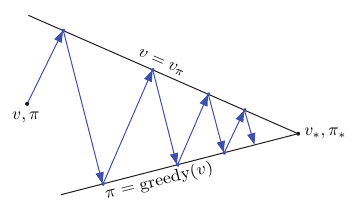
\includegraphics[width=0.5\linewidth]{GPI.png}
  \label{fig:GPI}
\end{figure}

For GPI examples, the value iteration only uses one sweep of policy evaluation. Almost all RL methods are GPI.

Monte Carlo sampling method, an alternative to learn a value function, estimates each state value independently by averaging large number of returns.
Brute-force search is an alternative for finding $\pi_*$ by computing with every $\pi$.
Bootstrapping, the process of using the value estimates of successor states to improve current value estimate. This is more efficient (estimating value collectively) than Monte Carlo method (estimating each value independently).

\subsection{Efficiency of Dynamic Programming}

DP, in the worst case, the time takes to find an optimal solution is polynomial in the number of states and actions (even though the total number of deterministic policies is $|\mathcal{A}|^{|\mathcal{S}|}$. DP is better at large state spaces than competing methods (e.g. direct search, linear programming).

\subsection{Summary}

\begin{itemize}
\item DP requires complete and accurate model of the environment
\item Policy evaluation: iterative computation of the value function for a given policy
\item Policy improvement: the computation of an improved policy (greedy operation) given the value function for that policy
\item Two most popular DP methods: policy iteration and value iteration, by combining policy evaluation and policy improvement. These two can solve finite MDPs given complete knowledge of the MDP
\item Classical DP: sweep whole state set, performing expected update on each state. The update is based on all possible successor states and their probabilities of occurring.
\item Generalized Policy Iteration (GPI): interacting processes (policy evaluation and policy improvement) revolving around an approximate policy and an approximate value function
\item Async DP: unlike classical/systematic DP, it update states in random order.
\item \textbf{bootstrapping}: update estimates on the basis of other estimates (English definition of bootstrap: you pull yourself up by your boot-straps, meaning you achieved success by your own efforts.)
\end{itemize}

\begin{table}[]
\begin{tabular}{l|l|l}
Problem                 & Bellman equation                                                                                    & Algorithm                   \\\hline
Prediction (evaluation) & Bellman Expectation Equation                                                                        & Iterative policy evaluation \\
Control                 & \begin{tabular}[c]{@{}l@{}}Bellman Expectation Equation + \\ Greedy Policy Improvement\end{tabular} & Policy Iteration            \\
Control                 & Bellman Optimality Equation                                                                         & Value Iteration            
\end{tabular}
\end{table}

\newpage
\subsection{Learning Objectives (UA RL MOOC)}

Only policies greedy with respect to the optimal value function are guaranteed to be optimal.

1. Understand the distinction between policy evaluation and control

policy evaluation computes the state value for $\pi$, while control is the dance of policy and value.

2. Explain the setting in which dynamic programming can be applied, as well as its limitations

DP can be applied in relatively large MDPs. Its limitations include (1) requiring complete model of the MDP.

3. Outline the iterative policy evaluation algorithm for estimating state values under a given policy

see chap 4.1

4. Apply iterative policy evaluation to compute value functions

5. Understand the policy improvement theorem

policy improvement theorem: the computation of an improved policy given the value function for that policy.

6. Use a value function for a policy to produce a better policy for a given MDP
7. Outline the policy iteration algorithm for finding the optimal policy

see chap 4.3

8. Understand “the dance of policy and value”

The PE and PI happens (mostly) alternatively, and reach optimal state value function and optimal policy eventually.

9. Apply policy iteration to compute optimal policies and optimal value functions

10. Understand the framework of generalized policy iteration

PE + PI. There can be multiple updates or no update for a state in each iteration. All state must be visited once.

11. Outline value iteration, an important example of generalized policy iteration

see chap 4.4

12. Understand the distinction between synchronous and asynchronous dynamic programming methods

sync DP is the systematic DP, which updates all states in order. async DP updates state in any order, which makes it for faster convergence.

13. Describe brute force search as an alternative method for searching for an optimal policy

Brute-force search takes $|A|^{|S|}$ time. It compute for every combination of state-action mappings (policies).

14. Describe Monte Carlo as an alternative method for learning a value function

MC estimates state value by averaging large number of returns.

15. Understand the advantage of Dynamic programming and “bootstrapping” over these alternative strategies for finding the optimal policy

DP is fast and bootstrapping uses more states' info during estimation than the other alternatives, which is more efficient.

16. Why are DP algorithms considered planning methods?

Because they use a model to improve the policy (which is the definition of planning method).


\end{document}